\documentclass[1p]{elsarticle_modified}
%\bibliographystyle{elsarticle-num}

%\usepackage[colorlinks]{hyperref}
%\usepackage{abbrmath_seonhwa} %\Abb, \Ascr, \Acal ,\Abf, \Afrak
\usepackage{amsfonts}
\usepackage{amssymb}
\usepackage{amsmath}
\usepackage{amsthm}
\usepackage{scalefnt}
\usepackage{amsbsy}
\usepackage{kotex}
\usepackage{caption}
\usepackage{subfig}
\usepackage{color}
\usepackage{graphicx}
\usepackage{xcolor} %% white, black, red, green, blue, cyan, magenta, yellow
\usepackage{float}
\usepackage{setspace}
\usepackage{hyperref}

\usepackage{tikz}
\usetikzlibrary{arrows}

\usepackage{multirow}
\usepackage{array} % fixed length table
\usepackage{hhline}

%%%%%%%%%%%%%%%%%%%%%
\makeatletter
\renewcommand*\env@matrix[1][\arraystretch]{%
	\edef\arraystretch{#1}%
	\hskip -\arraycolsep
	\let\@ifnextchar\new@ifnextchar
	\array{*\c@MaxMatrixCols c}}
\makeatother %https://tex.stackexchange.com/questions/14071/how-can-i-increase-the-line-spacing-in-a-matrix
%%%%%%%%%%%%%%%

\usepackage[normalem]{ulem}

\newcommand{\msout}[1]{\ifmmode\text{\sout{\ensuremath{#1}}}\else\sout{#1}\fi}
%SOURCE: \msout is \stkout macro in https://tex.stackexchange.com/questions/20609/strikeout-in-math-mode

\newcommand{\cancel}[1]{
	\ifmmode
	{\color{red}\msout{#1}}
	\else
	{\color{red}\sout{#1}}
	\fi
}

\newcommand{\add}[1]{
	{\color{blue}\uwave{#1}}
}

\newcommand{\replace}[2]{
	\ifmmode
	{\color{red}\msout{#1}}{\color{blue}\uwave{#2}}
	\else
	{\color{red}\sout{#1}}{\color{blue}\uwave{#2}}
	\fi
}

\newcommand{\Sol}{\mathcal{S}} %segment
\newcommand{\D}{D} %diagram
\newcommand{\A}{\mathcal{A}} %arc


%%%%%%%%%%%%%%%%%%%%%%%%%%%%%5 test

\def\sl{\operatorname{\textup{SL}}(2,\Cbb)}
\def\psl{\operatorname{\textup{PSL}}(2,\Cbb)}
\def\quan{\mkern 1mu \triangleright \mkern 1mu}

\theoremstyle{definition}
\newtheorem{thm}{Theorem}[section]
\newtheorem{prop}[thm]{Proposition}
\newtheorem{lem}[thm]{Lemma}
\newtheorem{ques}[thm]{Question}
\newtheorem{cor}[thm]{Corollary}
\newtheorem{defn}[thm]{Definition}
\newtheorem{exam}[thm]{Example}
\newtheorem{rmk}[thm]{Remark}
\newtheorem{alg}[thm]{Algorithm}

\newcommand{\I}{\sqrt{-1}}
\begin{document}

%\begin{frontmatter}
%
%\title{Boundary parabolic representations of knots up to 8 crossings}
%
%%% Group authors per affiliation:
%\author{Yunhi Cho} 
%\address{Department of Mathematics, University of Seoul, Seoul, Korea}
%\ead{yhcho@uos.ac.kr}
%
%
%\author{Seonhwa Kim} %\fnref{s_kim}}
%\address{Center for Geometry and Physics, Institute for Basic Science, Pohang, 37673, Korea}
%\ead{ryeona17@ibs.re.kr}
%
%\author{Hyuk Kim}
%\address{Department of Mathematical Sciences, Seoul National University, Seoul 08826, Korea}
%\ead{hyukkim@snu.ac.kr}
%
%\author{Seokbeom Yoon}
%\address{Department of Mathematical Sciences, Seoul National University, Seoul, 08826,  Korea}
%\ead{sbyoon15@snu.ac.kr}
%
%\begin{abstract}
%We find all boundary parabolic representation of knots up to 8 crossings.
%
%\end{abstract}
%\begin{keyword}
%    \MSC[2010] 57M25 
%\end{keyword}
%
%\end{frontmatter}

%\linenumbers
%\tableofcontents
%
\newcommand\colored[1]{\textcolor{white}{\rule[-0.35ex]{0.8em}{1.4ex}}\kern-0.8em\color{red} #1}%
%\newcommand\colored[1]{\textcolor{white}{ #1}\kern-2.17ex	\textcolor{white}{ #1}\kern-1.81ex	\textcolor{white}{ #1}\kern-2.15ex\color{red}#1	}

{\Large $\underline{12n_{0563}~(K12n_{0563})}$}

\setlength{\tabcolsep}{10pt}
\renewcommand{\arraystretch}{1.6}
\vspace{1cm}\begin{tabular}{m{100pt}>{\centering\arraybackslash}m{274pt}}
\multirow{5}{120pt}{
	\centering
	\includegraphics[width=112pt]{../../../GIT/diagram.site/Diagrams/png/2652_12n_0563.png}\\
\ \ \ A knot diagram\footnotemark}&
\allowdisplaybreaks
\textbf{Linearized knot diagam} \\
\cline{2-2}
 &
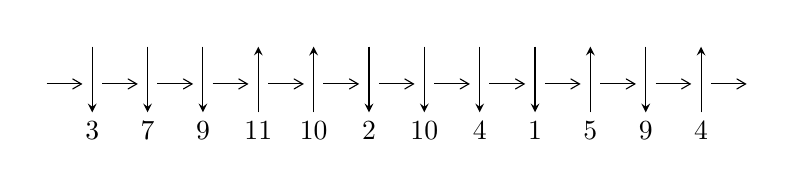
\begin{tikzpicture}[x=20pt, y=17pt]
	% nodes
	\node (C0) at (0, 0) {};
	\node (C1) at (1, 0) {};
	\node (C1U) at (1, +1) {};
	\node (C1D) at (1, -1) {3};

	\node (C2) at (2, 0) {};
	\node (C2U) at (2, +1) {};
	\node (C2D) at (2, -1) {7};

	\node (C3) at (3, 0) {};
	\node (C3U) at (3, +1) {};
	\node (C3D) at (3, -1) {9};

	\node (C4) at (4, 0) {};
	\node (C4U) at (4, +1) {};
	\node (C4D) at (4, -1) {11};

	\node (C5) at (5, 0) {};
	\node (C5U) at (5, +1) {};
	\node (C5D) at (5, -1) {10};

	\node (C6) at (6, 0) {};
	\node (C6U) at (6, +1) {};
	\node (C6D) at (6, -1) {2};

	\node (C7) at (7, 0) {};
	\node (C7U) at (7, +1) {};
	\node (C7D) at (7, -1) {10};

	\node (C8) at (8, 0) {};
	\node (C8U) at (8, +1) {};
	\node (C8D) at (8, -1) {4};

	\node (C9) at (9, 0) {};
	\node (C9U) at (9, +1) {};
	\node (C9D) at (9, -1) {1};

	\node (C10) at (10, 0) {};
	\node (C10U) at (10, +1) {};
	\node (C10D) at (10, -1) {5};

	\node (C11) at (11, 0) {};
	\node (C11U) at (11, +1) {};
	\node (C11D) at (11, -1) {9};

	\node (C12) at (12, 0) {};
	\node (C12U) at (12, +1) {};
	\node (C12D) at (12, -1) {4};
	\node (C13) at (13, 0) {};

	% arrows
	\draw[->,>={angle 60}]
	(C0) edge (C1) (C1) edge (C2) (C2) edge (C3) (C3) edge (C4) (C4) edge (C5) (C5) edge (C6) (C6) edge (C7) (C7) edge (C8) (C8) edge (C9) (C9) edge (C10) (C10) edge (C11) (C11) edge (C12) (C12) edge (C13) ;	\draw[->,>=stealth]
	(C1U) edge (C1D) (C2U) edge (C2D) (C3U) edge (C3D) (C4D) edge (C4U) (C5D) edge (C5U) (C6U) edge (C6D) (C7U) edge (C7D) (C8U) edge (C8D) (C9U) edge (C9D) (C10D) edge (C10U) (C11U) edge (C11D) (C12D) edge (C12U) ;
	\end{tikzpicture} \\
\hhline{~~} \\& 
\textbf{Solving Sequence} \\ \cline{2-2} 
 &
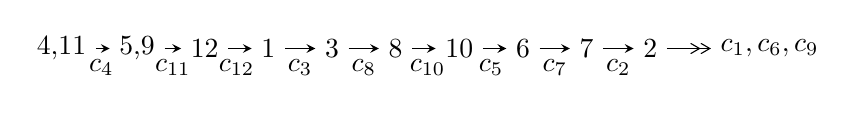
\begin{tikzpicture}[x=23pt, y=7pt]
	% node
	\node (A0) at (-1/8, 0) {4,11};
	\node (A1) at (17/16, 0) {5,9};
	\node (A2) at (17/8, 0) {12};
	\node (A3) at (25/8, 0) {1};
	\node (A4) at (33/8, 0) {3};
	\node (A5) at (41/8, 0) {8};
	\node (A6) at (49/8, 0) {10};
	\node (A7) at (57/8, 0) {6};
	\node (A8) at (65/8, 0) {7};
	\node (A9) at (73/8, 0) {2};
	\node (C1) at (1/2, -1) {$c_{4}$};
	\node (C2) at (13/8, -1) {$c_{11}$};
	\node (C3) at (21/8, -1) {$c_{12}$};
	\node (C4) at (29/8, -1) {$c_{3}$};
	\node (C5) at (37/8, -1) {$c_{8}$};
	\node (C6) at (45/8, -1) {$c_{10}$};
	\node (C7) at (53/8, -1) {$c_{5}$};
	\node (C8) at (61/8, -1) {$c_{7}$};
	\node (C9) at (69/8, -1) {$c_{2}$};
	\node (A10) at (11, 0) {$c_{1},c_{6},c_{9}$};

	% edge
	\draw[->,>=stealth]	
	(A0) edge (A1) (A1) edge (A2) (A2) edge (A3) (A3) edge (A4) (A4) edge (A5) (A5) edge (A6) (A6) edge (A7) (A7) edge (A8) (A8) edge (A9) ;
	\draw[->>,>={angle 60}]	
	(A9) edge (A10);
\end{tikzpicture} \\ 

\end{tabular} \\

\footnotetext{
The image of knot diagram is generated by the software ``\textbf{Draw programme}" developed by Andrew Bartholomew(\url{http://www.layer8.co.uk/maths/draw/index.htm\#Running-draw}), where we modified some parts for our purpose(\url{https://github.com/CATsTAILs/LinksPainter}).
}\phantom \\ \newline 
\centering \textbf{Ideals for irreducible components\footnotemark of $X_{\text{par}}$} 
 
\begin{align*}
I^u_{1}&=\langle 
-2.39160\times10^{54} u^{47}-3.95222\times10^{54} u^{46}+\cdots+7.49953\times10^{54} b-2.89856\times10^{55},\\
\phantom{I^u_{1}}&\phantom{= \langle  }1.44654\times10^{55} u^{47}-1.62245\times10^{55} u^{46}+\cdots+7.49953\times10^{54} a+4.83415\times10^{55},\;u^{48}- u^{47}+\cdots+3 u+1\rangle \\
I^u_{2}&=\langle 
- u^3+b-2 u,\;- u^{12}- u^{11}-8 u^{10}-7 u^9-25 u^8-17 u^7-39 u^6-17 u^5-32 u^4-6 u^3-14 u^2+a+u-4,\\
\phantom{I^u_{2}}&\phantom{= \langle  }u^{13}+8 u^{11}+25 u^9- u^8+40 u^7-5 u^6+36 u^5-8 u^4+18 u^3-5 u^2+5 u-1\rangle \\
\\
\end{align*}
\raggedright * 2 irreducible components of $\dim_{\mathbb{C}}=0$, with total 61 representations.\\
\footnotetext{All coefficients of polynomials are rational numbers. But the coefficients are sometimes approximated in decimal forms when there is not enough margin.}
\newpage
\renewcommand{\arraystretch}{1}
\centering \section*{I. $I^u_{1}= \langle -2.39\times10^{54} u^{47}-3.95\times10^{54} u^{46}+\cdots+7.50\times10^{54} b-2.90\times10^{55},\;1.45\times10^{55} u^{47}-1.62\times10^{55} u^{46}+\cdots+7.50\times10^{54} a+4.83\times10^{55},\;u^{48}- u^{47}+\cdots+3 u+1 \rangle$}
\flushleft \textbf{(i) Arc colorings}\\
\begin{tabular}{m{7pt} m{180pt} m{7pt} m{180pt} }
\flushright $a_{4}=$&$\begin{pmatrix}1\\0\end{pmatrix}$ \\
\flushright $a_{11}=$&$\begin{pmatrix}0\\u\end{pmatrix}$ \\
\flushright $a_{5}=$&$\begin{pmatrix}1\\- u^2\end{pmatrix}$ \\
\flushright $a_{9}=$&$\begin{pmatrix}-1.92884 u^{47}+2.16340 u^{46}+\cdots-4.69127 u-6.44593\\0.318900 u^{47}+0.526995 u^{46}+\cdots+7.68737 u+3.86499\end{pmatrix}$ \\
\flushright $a_{12}=$&$\begin{pmatrix}5.32722 u^{47}-7.71278 u^{46}+\cdots+5.69560 u+4.89101\\-1.65263 u^{47}+2.15021 u^{46}+\cdots-2.13909 u+0.429005\end{pmatrix}$ \\
\flushright $a_{1}=$&$\begin{pmatrix}3.67459 u^{47}-5.56258 u^{46}+\cdots+3.55651 u+5.32002\\-1.65263 u^{47}+2.15021 u^{46}+\cdots-2.13909 u+0.429005\end{pmatrix}$ \\
\flushright $a_{3}=$&$\begin{pmatrix}-0.429005 u^{47}-1.22363 u^{46}+\cdots-12.6538 u-3.42610\\-0.741759 u^{47}+0.279846 u^{46}+\cdots-3.69494 u+0.760160\end{pmatrix}$ \\
\flushright $a_{8}=$&$\begin{pmatrix}-1.60994 u^{47}+2.69040 u^{46}+\cdots+2.99610 u-2.58094\\0.318900 u^{47}+0.526995 u^{46}+\cdots+7.68737 u+3.86499\end{pmatrix}$ \\
\flushright $a_{10}=$&$\begin{pmatrix}- u\\u^3+u\end{pmatrix}$ \\
\flushright $a_{6}=$&$\begin{pmatrix}u^2+1\\- u^4-2 u^2\end{pmatrix}$ \\
\flushright $a_{7}=$&$\begin{pmatrix}-1.84566 u^{47}+2.55030 u^{46}+\cdots-1.55830 u-4.58260\\0.553995 u^{47}+0.491959 u^{46}+\cdots+10.8786 u+5.49084\end{pmatrix}$ \\
\flushright $a_{2}=$&$\begin{pmatrix}1.85623 u^{47}-3.48934 u^{46}+\cdots-4.22125 u+2.81550\\-0.399504 u^{47}-1.07854 u^{46}+\cdots-11.0873 u-2.93213\end{pmatrix}$\\&\end{tabular}
\flushleft \textbf{(ii) Obstruction class $= -1$}\\~\\
\flushleft \textbf{(iii) Cusp Shapes $= 7.73136 u^{47}-12.6807 u^{46}+\cdots-1.90430 u+10.9470$}\\~\\
\newpage\renewcommand{\arraystretch}{1}
\flushleft \textbf{(iv) u-Polynomials at the component}\newline \\
\begin{tabular}{m{50pt}|m{274pt}}
Crossings & \hspace{64pt}u-Polynomials at each crossing \\
\hline $$\begin{aligned}c_{1}\end{aligned}$$&$\begin{aligned}
&u^{48}+14 u^{47}+\cdots+1783 u+121
\end{aligned}$\\
\hline $$\begin{aligned}c_{2},c_{6}\end{aligned}$$&$\begin{aligned}
&u^{48}-2 u^{47}+\cdots-21 u-11
\end{aligned}$\\
\hline $$\begin{aligned}c_{3},c_{8}\end{aligned}$$&$\begin{aligned}
&u^{48}- u^{47}+\cdots+56 u-1
\end{aligned}$\\
\hline $$\begin{aligned}c_{4},c_{5},c_{10}\end{aligned}$$&$\begin{aligned}
&u^{48}- u^{47}+\cdots+3 u+1
\end{aligned}$\\
\hline $$\begin{aligned}c_{7}\end{aligned}$$&$\begin{aligned}
&u^{48}-8 u^{47}+\cdots-28403 u+7979
\end{aligned}$\\
\hline $$\begin{aligned}c_{9}\end{aligned}$$&$\begin{aligned}
&u^{48}+4 u^{47}+\cdots-231 u-49
\end{aligned}$\\
\hline $$\begin{aligned}c_{11}\end{aligned}$$&$\begin{aligned}
&u^{48}-2 u^{47}+\cdots+2483 u-169
\end{aligned}$\\
\hline $$\begin{aligned}c_{12}\end{aligned}$$&$\begin{aligned}
&u^{48}+5 u^{47}+\cdots+2615 u+313
\end{aligned}$\\
\hline
\end{tabular}\\~\\
\newpage\renewcommand{\arraystretch}{1}
\flushleft \textbf{(v) Riley Polynomials at the component}\newline \\
\begin{tabular}{m{50pt}|m{274pt}}
Crossings & \hspace{64pt}Riley Polynomials at each crossing \\
\hline $$\begin{aligned}c_{1}\end{aligned}$$&$\begin{aligned}
&y^{48}+46 y^{47}+\cdots+485517 y+14641
\end{aligned}$\\
\hline $$\begin{aligned}c_{2},c_{6}\end{aligned}$$&$\begin{aligned}
&y^{48}-14 y^{47}+\cdots-1783 y+121
\end{aligned}$\\
\hline $$\begin{aligned}c_{3},c_{8}\end{aligned}$$&$\begin{aligned}
&y^{48}+55 y^{47}+\cdots-3490 y+1
\end{aligned}$\\
\hline $$\begin{aligned}c_{4},c_{5},c_{10}\end{aligned}$$&$\begin{aligned}
&y^{48}+35 y^{47}+\cdots- y+1
\end{aligned}$\\
\hline $$\begin{aligned}c_{7}\end{aligned}$$&$\begin{aligned}
&y^{48}+46 y^{47}+\cdots+1653354871 y+63664441
\end{aligned}$\\
\hline $$\begin{aligned}c_{9}\end{aligned}$$&$\begin{aligned}
&y^{48}+2 y^{47}+\cdots+7105 y+2401
\end{aligned}$\\
\hline $$\begin{aligned}c_{11}\end{aligned}$$&$\begin{aligned}
&y^{48}+58 y^{47}+\cdots-2857283 y+28561
\end{aligned}$\\
\hline $$\begin{aligned}c_{12}\end{aligned}$$&$\begin{aligned}
&y^{48}-69 y^{47}+\cdots-5964955 y+97969
\end{aligned}$\\
\hline
\end{tabular}\\~\\
\newpage\flushleft \textbf{(vi) Complex Volumes and Cusp Shapes}
$$\begin{array}{c|c|c}  
\text{Solutions to }I^u_{1}& \I (\text{vol} + \sqrt{-1}CS) & \text{Cusp shape}\\
 \hline 
\begin{aligned}
u &= -0.435520 + 0.942072 I \\
a &= -1.076810 - 0.546005 I \\
b &= -0.075623 - 0.253208 I\end{aligned}
 & \phantom{-}0.84017 + 1.53001 I & -4.48166 - 1.67187 I \\ \hline\begin{aligned}
u &= -0.435520 - 0.942072 I \\
a &= -1.076810 + 0.546005 I \\
b &= -0.075623 + 0.253208 I\end{aligned}
 & \phantom{-}0.84017 - 1.53001 I & -4.48166 + 1.67187 I \\ \hline\begin{aligned}
u &= -0.154361 + 1.095650 I \\
a &= \phantom{-}0.750842 - 0.363346 I \\
b &= \phantom{-}0.920518 - 0.093530 I\end{aligned}
 & -4.71668 - 2.11923 I & -10.82328 + 3.73003 I \\ \hline\begin{aligned}
u &= -0.154361 - 1.095650 I \\
a &= \phantom{-}0.750842 + 0.363346 I \\
b &= \phantom{-}0.920518 + 0.093530 I\end{aligned}
 & -4.71668 + 2.11923 I & -10.82328 - 3.73003 I \\ \hline\begin{aligned}
u &= \phantom{-}0.443963 + 1.034950 I \\
a &= -0.551533 - 0.438377 I \\
b &= -1.052700 + 0.633094 I\end{aligned}
 & \phantom{-}1.19625 + 2.65861 I & -4.00000 - 4.52024 I \\ \hline\begin{aligned}
u &= \phantom{-}0.443963 - 1.034950 I \\
a &= -0.551533 + 0.438377 I \\
b &= -1.052700 - 0.633094 I\end{aligned}
 & \phantom{-}1.19625 - 2.65861 I & -4.00000 + 4.52024 I \\ \hline\begin{aligned}
u &= -0.376782 + 0.764505 I \\
a &= -1.67330 + 2.06393 I \\
b &= -0.050763 - 1.300670 I\end{aligned}
 & \phantom{-}4.54023 - 1.72963 I & \phantom{-}4.64800 + 3.11123 I \\ \hline\begin{aligned}
u &= -0.376782 - 0.764505 I \\
a &= -1.67330 - 2.06393 I \\
b &= -0.050763 + 1.300670 I\end{aligned}
 & \phantom{-}4.54023 + 1.72963 I & \phantom{-}4.64800 - 3.11123 I \\ \hline\begin{aligned}
u &= \phantom{-}0.625304 + 0.996638 I \\
a &= -0.815699 - 0.738147 I \\
b &= -0.21810 + 1.41293 I\end{aligned}
 & \phantom{-}1.47522 + 0.81061 I & \phantom{-0.000000 } 0 \\ \hline\begin{aligned}
u &= \phantom{-}0.625304 - 0.996638 I \\
a &= -0.815699 + 0.738147 I \\
b &= -0.21810 - 1.41293 I\end{aligned}
 & \phantom{-}1.47522 - 0.81061 I & \phantom{-0.000000 } 0\\
 \hline 
 \end{array}$$\newpage$$\begin{array}{c|c|c}  
\text{Solutions to }I^u_{1}& \I (\text{vol} + \sqrt{-1}CS) & \text{Cusp shape}\\
 \hline 
\begin{aligned}
u &= -1.179960 + 0.123958 I \\
a &= -0.19080 + 1.69727 I \\
b &= \phantom{-}0.16078 - 1.62361 I\end{aligned}
 & \phantom{-}11.96410 + 1.32500 I & \phantom{-0.000000 } 0 \\ \hline\begin{aligned}
u &= -1.179960 - 0.123958 I \\
a &= -0.19080 - 1.69727 I \\
b &= \phantom{-}0.16078 + 1.62361 I\end{aligned}
 & \phantom{-}11.96410 - 1.32500 I & \phantom{-0.000000 } 0 \\ \hline\begin{aligned}
u &= -0.269250 + 1.162830 I \\
a &= \phantom{-}0.839939 - 0.658536 I \\
b &= \phantom{-}0.20024 + 1.60053 I\end{aligned}
 & \phantom{-}1.26689 - 2.36269 I & \phantom{-0.000000 } 0 \\ \hline\begin{aligned}
u &= -0.269250 - 1.162830 I \\
a &= \phantom{-}0.839939 + 0.658536 I \\
b &= \phantom{-}0.20024 - 1.60053 I\end{aligned}
 & \phantom{-}1.26689 + 2.36269 I & \phantom{-0.000000 } 0 \\ \hline\begin{aligned}
u &= -0.427605 + 1.128960 I \\
a &= \phantom{-}0.534297 - 0.374229 I \\
b &= \phantom{-}1.308210 + 0.533677 I\end{aligned}
 & \phantom{-}0.10991 - 8.23975 I & \phantom{-0.000000 } 0 \\ \hline\begin{aligned}
u &= -0.427605 - 1.128960 I \\
a &= \phantom{-}0.534297 + 0.374229 I \\
b &= \phantom{-}1.308210 - 0.533677 I\end{aligned}
 & \phantom{-}0.10991 + 8.23975 I & \phantom{-0.000000 } 0 \\ \hline\begin{aligned}
u &= \phantom{-}0.352885 + 1.172480 I \\
a &= \phantom{-}1.53487 + 0.77490 I \\
b &= \phantom{-}0.397307 - 1.278340 I\end{aligned}
 & -0.92113 + 6.80242 I & \phantom{-0.000000 } 0 \\ \hline\begin{aligned}
u &= \phantom{-}0.352885 - 1.172480 I \\
a &= \phantom{-}1.53487 - 0.77490 I \\
b &= \phantom{-}0.397307 + 1.278340 I\end{aligned}
 & -0.92113 - 6.80242 I & \phantom{-0.000000 } 0 \\ \hline\begin{aligned}
u &= \phantom{-}1.226860 + 0.007840 I \\
a &= \phantom{-}0.12427 + 1.63006 I \\
b &= -0.18772 - 1.63918 I\end{aligned}
 & \phantom{-}11.45140 - 7.76917 I & \phantom{-0.000000 } 0 \\ \hline\begin{aligned}
u &= \phantom{-}1.226860 - 0.007840 I \\
a &= \phantom{-}0.12427 - 1.63006 I \\
b &= -0.18772 + 1.63918 I\end{aligned}
 & \phantom{-}11.45140 + 7.76917 I & \phantom{-0.000000 } 0\\
 \hline 
 \end{array}$$\newpage$$\begin{array}{c|c|c}  
\text{Solutions to }I^u_{1}& \I (\text{vol} + \sqrt{-1}CS) & \text{Cusp shape}\\
 \hline 
\begin{aligned}
u &= \phantom{-}0.376298 + 1.187320 I \\
a &= \phantom{-}0.913505 - 0.477894 I \\
b &= \phantom{-}0.057189 - 0.405233 I\end{aligned}
 & \phantom{-}0.12397 + 4.49470 I & \phantom{-0.000000 } 0 \\ \hline\begin{aligned}
u &= \phantom{-}0.376298 - 1.187320 I \\
a &= \phantom{-}0.913505 + 0.477894 I \\
b &= \phantom{-}0.057189 + 0.405233 I\end{aligned}
 & \phantom{-}0.12397 - 4.49470 I & \phantom{-0.000000 } 0 \\ \hline\begin{aligned}
u &= \phantom{-}0.580032 + 0.452436 I \\
a &= -0.92293 - 1.44096 I \\
b &= -0.33652 + 1.50463 I\end{aligned}
 & \phantom{-}2.95847 + 4.00692 I & -2.67836 - 6.96933 I \\ \hline\begin{aligned}
u &= \phantom{-}0.580032 - 0.452436 I \\
a &= -0.92293 + 1.44096 I \\
b &= -0.33652 - 1.50463 I\end{aligned}
 & \phantom{-}2.95847 - 4.00692 I & -2.67836 + 6.96933 I \\ \hline\begin{aligned}
u &= -0.151969 + 0.640678 I \\
a &= \phantom{-}1.79473 + 2.00434 I \\
b &= -0.128016 - 1.103990 I\end{aligned}
 & \phantom{-}2.23261 - 4.69663 I & -2.29866 + 7.37362 I \\ \hline\begin{aligned}
u &= -0.151969 - 0.640678 I \\
a &= \phantom{-}1.79473 - 2.00434 I \\
b &= -0.128016 + 1.103990 I\end{aligned}
 & \phantom{-}2.23261 + 4.69663 I & -2.29866 - 7.37362 I \\ \hline\begin{aligned}
u &= -0.024639 + 0.631913 I \\
a &= \phantom{-}1.292480 - 0.327555 I \\
b &= \phantom{-}0.44857 + 1.55247 I\end{aligned}
 & \phantom{-}3.50058 + 0.55008 I & -1.118536 - 0.349377 I \\ \hline\begin{aligned}
u &= -0.024639 - 0.631913 I \\
a &= \phantom{-}1.292480 + 0.327555 I \\
b &= \phantom{-}0.44857 - 1.55247 I\end{aligned}
 & \phantom{-}3.50058 - 0.55008 I & -1.118536 + 0.349377 I \\ \hline\begin{aligned}
u &= \phantom{-}0.219879 + 0.581123 I \\
a &= -0.507645 - 0.541214 I \\
b &= -0.194376 + 0.350188 I\end{aligned}
 & -0.254703 + 1.031080 I & -4.07316 - 6.58896 I \\ \hline\begin{aligned}
u &= \phantom{-}0.219879 - 0.581123 I \\
a &= -0.507645 + 0.541214 I \\
b &= -0.194376 - 0.350188 I\end{aligned}
 & -0.254703 - 1.031080 I & -4.07316 + 6.58896 I\\
 \hline 
 \end{array}$$\newpage$$\begin{array}{c|c|c}  
\text{Solutions to }I^u_{1}& \I (\text{vol} + \sqrt{-1}CS) & \text{Cusp shape}\\
 \hline 
\begin{aligned}
u &= -0.65049 + 1.32174 I \\
a &= -0.96287 + 1.04566 I \\
b &= -0.36043 - 1.58899 I\end{aligned}
 & \phantom{-}8.28567 - 7.72804 I & \phantom{-0.000000 } 0 \\ \hline\begin{aligned}
u &= -0.65049 - 1.32174 I \\
a &= -0.96287 - 1.04566 I \\
b &= -0.36043 + 1.58899 I\end{aligned}
 & \phantom{-}8.28567 + 7.72804 I & \phantom{-0.000000 } 0 \\ \hline\begin{aligned}
u &= -0.08747 + 1.49239 I \\
a &= \phantom{-}0.207043 + 0.731169 I \\
b &= -0.048453 - 0.802768 I\end{aligned}
 & -7.65194 - 1.77181 I & \phantom{-0.000000 } 0 \\ \hline\begin{aligned}
u &= -0.08747 - 1.49239 I \\
a &= \phantom{-}0.207043 - 0.731169 I \\
b &= -0.048453 + 0.802768 I\end{aligned}
 & -7.65194 + 1.77181 I & \phantom{-0.000000 } 0 \\ \hline\begin{aligned}
u &= \phantom{-}0.498135 + 0.056251 I \\
a &= -1.178220 + 0.256245 I \\
b &= \phantom{-}0.343725 + 0.931868 I\end{aligned}
 & \phantom{-}3.49281 + 1.01877 I & \phantom{-}0.423557 - 0.776578 I \\ \hline\begin{aligned}
u &= \phantom{-}0.498135 - 0.056251 I \\
a &= -1.178220 - 0.256245 I \\
b &= \phantom{-}0.343725 - 0.931868 I\end{aligned}
 & \phantom{-}3.49281 - 1.01877 I & \phantom{-}0.423557 + 0.776578 I \\ \hline\begin{aligned}
u &= \phantom{-}0.62518 + 1.40469 I \\
a &= \phantom{-}0.905325 + 0.965225 I \\
b &= \phantom{-}0.41416 - 1.62727 I\end{aligned}
 & \phantom{-}7.1315 + 14.2674 I & \phantom{-0.000000 } 0 \\ \hline\begin{aligned}
u &= \phantom{-}0.62518 - 1.40469 I \\
a &= \phantom{-}0.905325 - 0.965225 I \\
b &= \phantom{-}0.41416 + 1.62727 I\end{aligned}
 & \phantom{-}7.1315 - 14.2674 I & \phantom{-0.000000 } 0 \\ \hline\begin{aligned}
u &= -0.382314 + 0.212503 I \\
a &= \phantom{-}0.083866 + 0.833170 I \\
b &= -0.701403 + 1.054330 I\end{aligned}
 & \phantom{-}2.71637 + 4.57604 I & -0.11105 - 6.10786 I \\ \hline\begin{aligned}
u &= -0.382314 - 0.212503 I \\
a &= \phantom{-}0.083866 - 0.833170 I \\
b &= -0.701403 - 1.054330 I\end{aligned}
 & \phantom{-}2.71637 - 4.57604 I & -0.11105 + 6.10786 I\\
 \hline 
 \end{array}$$\newpage$$\begin{array}{c|c|c}  
\text{Solutions to }I^u_{1}& \I (\text{vol} + \sqrt{-1}CS) & \text{Cusp shape}\\
 \hline 
\begin{aligned}
u &= -0.426711\phantom{ +0.000000I} \\
a &= \phantom{-}0.214040\phantom{ +0.000000I} \\
b &= -0.725860\phantom{ +0.000000I}\end{aligned}
 & -1.65788\phantom{ +0.000000I} & -3.70660\phantom{ +0.000000I} \\ \hline\begin{aligned}
u &= -0.404609\phantom{ +0.000000I} \\
a &= -2.82616\phantom{ +0.000000I} \\
b &= \phantom{-}0.0167904\phantom{ +0.000000I}\end{aligned}
 & -2.55057\phantom{ +0.000000I} & \phantom{-}7.13390\phantom{ +0.000000I} \\ \hline\begin{aligned}
u &= \phantom{-}0.66628 + 1.45057 I \\
a &= -0.816215 - 0.730920 I \\
b &= -0.03431 + 1.50514 I\end{aligned}
 & \phantom{-}6.99328 - 1.08384 I & \phantom{-0.000000 } 0 \\ \hline\begin{aligned}
u &= \phantom{-}0.66628 - 1.45057 I \\
a &= -0.816215 + 0.730920 I \\
b &= -0.03431 - 1.50514 I\end{aligned}
 & \phantom{-}6.99328 + 1.08384 I & \phantom{-0.000000 } 0 \\ \hline\begin{aligned}
u &= -0.57241 + 1.49585 I \\
a &= \phantom{-}0.805241 - 0.729040 I \\
b &= \phantom{-}0.03707 + 1.53975 I\end{aligned}
 & \phantom{-}6.90676 - 4.94555 I & \phantom{-0.000000 } 0 \\ \hline\begin{aligned}
u &= -0.57241 - 1.49585 I \\
a &= \phantom{-}0.805241 + 0.729040 I \\
b &= \phantom{-}0.03707 - 1.53975 I\end{aligned}
 & \phantom{-}6.90676 + 4.94555 I & \phantom{-0.000000 } 0 \\ \hline\begin{aligned}
u &= \phantom{-}0.01361 + 1.60580 I \\
a &= \phantom{-}0.215681 + 0.206965 I \\
b &= -0.044827 - 0.676036 I\end{aligned}
 & -8.07717 + 1.45463 I & \phantom{-0.000000 } 0 \\ \hline\begin{aligned}
u &= \phantom{-}0.01361 - 1.60580 I \\
a &= \phantom{-}0.215681 - 0.206965 I \\
b &= -0.044827 + 0.676036 I\end{aligned}
 & -8.07717 - 1.45463 I & \phantom{-0.000000 } 0\\
 \hline 
 \end{array}$$\newpage\newpage\renewcommand{\arraystretch}{1}
\centering \section*{II. $I^u_{2}= \langle - u^3+b-2 u,\;- u^{12}- u^{11}+\cdots+a-4,\;u^{13}+8 u^{11}+\cdots+5 u-1 \rangle$}
\flushleft \textbf{(i) Arc colorings}\\
\begin{tabular}{m{7pt} m{180pt} m{7pt} m{180pt} }
\flushright $a_{4}=$&$\begin{pmatrix}1\\0\end{pmatrix}$ \\
\flushright $a_{11}=$&$\begin{pmatrix}0\\u\end{pmatrix}$ \\
\flushright $a_{5}=$&$\begin{pmatrix}1\\- u^2\end{pmatrix}$ \\
\flushright $a_{9}=$&$\begin{pmatrix}u^{12}+u^{11}+\cdots- u+4\\u^3+2 u\end{pmatrix}$ \\
\flushright $a_{12}=$&$\begin{pmatrix}- u^{12}- u^{11}+\cdots-3 u-3\\u^{11}+7 u^9+18 u^7- u^6+22 u^5-4 u^4+14 u^3-4 u^2+4 u-1\end{pmatrix}$ \\
\flushright $a_{1}=$&$\begin{pmatrix}- u^{12}-8 u^{10}+\cdots+u-4\\u^{11}+7 u^9+18 u^7- u^6+22 u^5-4 u^4+14 u^3-4 u^2+4 u-1\end{pmatrix}$ \\
\flushright $a_{3}=$&$\begin{pmatrix}- u^{12}-7 u^{10}-18 u^8+u^7-22 u^6+4 u^5-14 u^4+4 u^3-4 u^2+u-1\\- u^6-4 u^4-4 u^2\end{pmatrix}$ \\
\flushright $a_{8}=$&$\begin{pmatrix}u^{12}+u^{11}+\cdots+u+4\\u^3+2 u\end{pmatrix}$ \\
\flushright $a_{10}=$&$\begin{pmatrix}- u\\u^3+u\end{pmatrix}$ \\
\flushright $a_{6}=$&$\begin{pmatrix}u^2+1\\- u^4-2 u^2\end{pmatrix}$ \\
\flushright $a_{7}=$&$\begin{pmatrix}u^{12}+u^{11}+\cdots+2 u+4\\- u^9-5 u^7-8 u^5-4 u^3+u\end{pmatrix}$ \\
\flushright $a_{2}=$&$\begin{pmatrix}- u^{12}-8 u^{10}-25 u^8+u^7-40 u^6+5 u^5-36 u^4+7 u^3-18 u^2+3 u-5\\- u^{11}-7 u^9-18 u^7-21 u^5-11 u^3- u\end{pmatrix}$\\&\end{tabular}
\flushleft \textbf{(ii) Obstruction class $= 1$}\\~\\
\flushleft \textbf{(iii) Cusp Shapes $= -2 u^{11}-5 u^{10}-15 u^9-30 u^8-42 u^7-65 u^6-51 u^5-68 u^4-23 u^3-38 u^2-2 u-16$}\\~\\
\newpage\renewcommand{\arraystretch}{1}
\flushleft \textbf{(iv) u-Polynomials at the component}\newline \\
\begin{tabular}{m{50pt}|m{274pt}}
Crossings & \hspace{64pt}u-Polynomials at each crossing \\
\hline $$\begin{aligned}c_{1}\end{aligned}$$&$\begin{aligned}
&u^{13}-5 u^{12}+\cdots+5 u-1
\end{aligned}$\\
\hline $$\begin{aligned}c_{2}\end{aligned}$$&$\begin{aligned}
&u^{13}- u^{12}+\cdots+u-1
\end{aligned}$\\
\hline $$\begin{aligned}c_{3}\end{aligned}$$&$\begin{aligned}
&u^{13}+8 u^{11}+\cdots+2 u-3
\end{aligned}$\\
\hline $$\begin{aligned}c_{4},c_{5}\end{aligned}$$&$\begin{aligned}
&u^{13}+8 u^{11}+\cdots+5 u-1
\end{aligned}$\\
\hline $$\begin{aligned}c_{6}\end{aligned}$$&$\begin{aligned}
&u^{13}+u^{12}+\cdots+u+1
\end{aligned}$\\
\hline $$\begin{aligned}c_{7}\end{aligned}$$&$\begin{aligned}
&u^{13}+3 u^{12}+\cdots-3 u-1
\end{aligned}$\\
\hline $$\begin{aligned}c_{8}\end{aligned}$$&$\begin{aligned}
&u^{13}+8 u^{11}+\cdots+2 u+3
\end{aligned}$\\
\hline $$\begin{aligned}c_{9}\end{aligned}$$&$\begin{aligned}
&u^{13}+3 u^{12}-4 u^{10}+2 u^9+u^8-4 u^7+3 u^6- u^5-2 u^4+2 u^3-2 u^2+u-1
\end{aligned}$\\
\hline $$\begin{aligned}c_{10}\end{aligned}$$&$\begin{aligned}
&u^{13}+8 u^{11}+\cdots+5 u+1
\end{aligned}$\\
\hline $$\begin{aligned}c_{11}\end{aligned}$$&$\begin{aligned}
&u^{13}+u^{12}+\cdots-3 u+1
\end{aligned}$\\
\hline $$\begin{aligned}c_{12}\end{aligned}$$&$\begin{aligned}
&u^{13}-2 u^{11}+3 u^{10}+3 u^9+u^8+10 u^7+2 u^6-4 u^5+5 u^4-2 u^3+5 u-1
\end{aligned}$\\
\hline
\end{tabular}\\~\\
\newpage\renewcommand{\arraystretch}{1}
\flushleft \textbf{(v) Riley Polynomials at the component}\newline \\
\begin{tabular}{m{50pt}|m{274pt}}
Crossings & \hspace{64pt}Riley Polynomials at each crossing \\
\hline $$\begin{aligned}c_{1}\end{aligned}$$&$\begin{aligned}
&y^{13}+11 y^{12}+\cdots-7 y-1
\end{aligned}$\\
\hline $$\begin{aligned}c_{2},c_{6}\end{aligned}$$&$\begin{aligned}
&y^{13}-5 y^{12}+\cdots+5 y-1
\end{aligned}$\\
\hline $$\begin{aligned}c_{3},c_{8}\end{aligned}$$&$\begin{aligned}
&y^{13}+16 y^{12}+\cdots-20 y-9
\end{aligned}$\\
\hline $$\begin{aligned}c_{4},c_{5},c_{10}\end{aligned}$$&$\begin{aligned}
&y^{13}+16 y^{12}+\cdots+15 y-1
\end{aligned}$\\
\hline $$\begin{aligned}c_{7}\end{aligned}$$&$\begin{aligned}
&y^{13}- y^{12}+\cdots+3 y-1
\end{aligned}$\\
\hline $$\begin{aligned}c_{9}\end{aligned}$$&$\begin{aligned}
&y^{13}-9 y^{12}+\cdots-3 y-1
\end{aligned}$\\
\hline $$\begin{aligned}c_{11}\end{aligned}$$&$\begin{aligned}
&y^{13}+3 y^{12}+\cdots+9 y-1
\end{aligned}$\\
\hline $$\begin{aligned}c_{12}\end{aligned}$$&$\begin{aligned}
&y^{13}-4 y^{12}+\cdots+25 y-1
\end{aligned}$\\
\hline
\end{tabular}\\~\\
\newpage\flushleft \textbf{(vi) Complex Volumes and Cusp Shapes}
$$\begin{array}{c|c|c}  
\text{Solutions to }I^u_{2}& \I (\text{vol} + \sqrt{-1}CS) & \text{Cusp shape}\\
 \hline 
\begin{aligned}
u &= -0.406397 + 0.828070 I \\
a &= \phantom{-}0.623860 - 1.154070 I \\
b &= -0.04391 + 1.49862 I\end{aligned}
 & \phantom{-}3.19757 - 2.07962 I & -2.23765 + 3.84644 I \\ \hline\begin{aligned}
u &= -0.406397 - 0.828070 I \\
a &= \phantom{-}0.623860 + 1.154070 I \\
b &= -0.04391 - 1.49862 I\end{aligned}
 & \phantom{-}3.19757 + 2.07962 I & -2.23765 - 3.84644 I \\ \hline\begin{aligned}
u &= -0.405399 + 1.034180 I \\
a &= \phantom{-}0.943206 - 0.498481 I \\
b &= \phantom{-}0.42334 + 1.47217 I\end{aligned}
 & \phantom{-}2.52863 - 1.04333 I & -0.891974 + 0.899946 I \\ \hline\begin{aligned}
u &= -0.405399 - 1.034180 I \\
a &= \phantom{-}0.943206 + 0.498481 I \\
b &= \phantom{-}0.42334 - 1.47217 I\end{aligned}
 & \phantom{-}2.52863 + 1.04333 I & -0.891974 - 0.899946 I \\ \hline\begin{aligned}
u &= \phantom{-}0.276046 + 1.147950 I \\
a &= -1.238510 + 0.159643 I \\
b &= -0.518180 + 1.045570 I\end{aligned}
 & \phantom{-}0.33288 + 6.03810 I & -3.21578 - 6.43497 I \\ \hline\begin{aligned}
u &= \phantom{-}0.276046 - 1.147950 I \\
a &= -1.238510 - 0.159643 I \\
b &= -0.518180 - 1.045570 I\end{aligned}
 & \phantom{-}0.33288 - 6.03810 I & -3.21578 + 6.43497 I \\ \hline\begin{aligned}
u &= \phantom{-}0.351249 + 0.612687 I \\
a &= -0.00263 - 1.64078 I \\
b &= \phantom{-}0.350273 + 1.222150 I\end{aligned}
 & \phantom{-}2.13932 - 3.61205 I & -3.50656 + 0.16807 I \\ \hline\begin{aligned}
u &= \phantom{-}0.351249 - 0.612687 I \\
a &= -0.00263 + 1.64078 I \\
b &= \phantom{-}0.350273 - 1.222150 I\end{aligned}
 & \phantom{-}2.13932 + 3.61205 I & -3.50656 - 0.16807 I \\ \hline\begin{aligned}
u &= \phantom{-}0.05874 + 1.54134 I \\
a &= -0.078914 + 0.461676 I \\
b &= -0.300983 - 0.563189 I\end{aligned}
 & -8.64883 + 1.03612 I & -15.2263 + 1.7097 I \\ \hline\begin{aligned}
u &= \phantom{-}0.05874 - 1.54134 I \\
a &= -0.078914 - 0.461676 I \\
b &= -0.300983 + 0.563189 I\end{aligned}
 & -8.64883 - 1.03612 I & -15.2263 - 1.7097 I\\
 \hline 
 \end{array}$$\newpage$$\begin{array}{c|c|c}  
\text{Solutions to }I^u_{2}& \I (\text{vol} + \sqrt{-1}CS) & \text{Cusp shape}\\
 \hline 
\begin{aligned}
u &= \phantom{-}0.02035 + 1.65258 I \\
a &= -0.017867 + 0.348906 I \\
b &= -0.126034 - 1.206020 I\end{aligned}
 & -6.33652 - 2.53081 I & -3.17775 + 4.10072 I \\ \hline\begin{aligned}
u &= \phantom{-}0.02035 - 1.65258 I \\
a &= -0.017867 - 0.348906 I \\
b &= -0.126034 + 1.206020 I\end{aligned}
 & -6.33652 + 2.53081 I & -3.17775 - 4.10072 I \\ \hline\begin{aligned}
u &= \phantom{-}0.210812\phantom{ +0.000000I} \\
a &= \phantom{-}4.54171\phantom{ +0.000000I} \\
b &= \phantom{-}0.430994\phantom{ +0.000000I}\end{aligned}
 & -2.87546\phantom{ +0.000000I} & -18.4880\phantom{ +0.000000I}\\
 \hline 
 \end{array}$$\newpage
\newpage\renewcommand{\arraystretch}{1}
\centering \section*{ III. u-Polynomials}
\begin{tabular}{m{50pt}|m{274pt}}
Crossings & \hspace{64pt}u-Polynomials at each crossing \\
\hline $$\begin{aligned}c_{1}\end{aligned}$$&$\begin{aligned}
&(u^{13}-5 u^{12}+\cdots+5 u-1)(u^{48}+14 u^{47}+\cdots+1783 u+121)
\end{aligned}$\\
\hline $$\begin{aligned}c_{2}\end{aligned}$$&$\begin{aligned}
&(u^{13}- u^{12}+\cdots+u-1)(u^{48}-2 u^{47}+\cdots-21 u-11)
\end{aligned}$\\
\hline $$\begin{aligned}c_{3}\end{aligned}$$&$\begin{aligned}
&(u^{13}+8 u^{11}+\cdots+2 u-3)(u^{48}- u^{47}+\cdots+56 u-1)
\end{aligned}$\\
\hline $$\begin{aligned}c_{4},c_{5}\end{aligned}$$&$\begin{aligned}
&(u^{13}+8 u^{11}+\cdots+5 u-1)(u^{48}- u^{47}+\cdots+3 u+1)
\end{aligned}$\\
\hline $$\begin{aligned}c_{6}\end{aligned}$$&$\begin{aligned}
&(u^{13}+u^{12}+\cdots+u+1)(u^{48}-2 u^{47}+\cdots-21 u-11)
\end{aligned}$\\
\hline $$\begin{aligned}c_{7}\end{aligned}$$&$\begin{aligned}
&(u^{13}+3 u^{12}+\cdots-3 u-1)(u^{48}-8 u^{47}+\cdots-28403 u+7979)
\end{aligned}$\\
\hline $$\begin{aligned}c_{8}\end{aligned}$$&$\begin{aligned}
&(u^{13}+8 u^{11}+\cdots+2 u+3)(u^{48}- u^{47}+\cdots+56 u-1)
\end{aligned}$\\
\hline $$\begin{aligned}c_{9}\end{aligned}$$&$\begin{aligned}
&(u^{13}+3 u^{12}-4 u^{10}+2 u^9+u^8-4 u^7+3 u^6- u^5-2 u^4+2 u^3-2 u^2+u-1)\\
&\cdot(u^{48}+4 u^{47}+\cdots-231 u-49)
\end{aligned}$\\
\hline $$\begin{aligned}c_{10}\end{aligned}$$&$\begin{aligned}
&(u^{13}+8 u^{11}+\cdots+5 u+1)(u^{48}- u^{47}+\cdots+3 u+1)
\end{aligned}$\\
\hline $$\begin{aligned}c_{11}\end{aligned}$$&$\begin{aligned}
&(u^{13}+u^{12}+\cdots-3 u+1)(u^{48}-2 u^{47}+\cdots+2483 u-169)
\end{aligned}$\\
\hline $$\begin{aligned}c_{12}\end{aligned}$$&$\begin{aligned}
&(u^{13}-2 u^{11}+3 u^{10}+3 u^9+u^8+10 u^7+2 u^6-4 u^5+5 u^4-2 u^3+5 u-1)\\
&\cdot(u^{48}+5 u^{47}+\cdots+2615 u+313)
\end{aligned}$\\
\hline
\end{tabular}\newpage\renewcommand{\arraystretch}{1}
\centering \section*{ IV. Riley Polynomials}
\begin{tabular}{m{50pt}|m{274pt}}
Crossings & \hspace{64pt}Riley Polynomials at each crossing \\
\hline $$\begin{aligned}c_{1}\end{aligned}$$&$\begin{aligned}
&(y^{13}+11 y^{12}+\cdots-7 y-1)(y^{48}+46 y^{47}+\cdots+485517 y+14641)
\end{aligned}$\\
\hline $$\begin{aligned}c_{2},c_{6}\end{aligned}$$&$\begin{aligned}
&(y^{13}-5 y^{12}+\cdots+5 y-1)(y^{48}-14 y^{47}+\cdots-1783 y+121)
\end{aligned}$\\
\hline $$\begin{aligned}c_{3},c_{8}\end{aligned}$$&$\begin{aligned}
&(y^{13}+16 y^{12}+\cdots-20 y-9)(y^{48}+55 y^{47}+\cdots-3490 y+1)
\end{aligned}$\\
\hline $$\begin{aligned}c_{4},c_{5},c_{10}\end{aligned}$$&$\begin{aligned}
&(y^{13}+16 y^{12}+\cdots+15 y-1)(y^{48}+35 y^{47}+\cdots- y+1)
\end{aligned}$\\
\hline $$\begin{aligned}c_{7}\end{aligned}$$&$\begin{aligned}
&(y^{13}- y^{12}+\cdots+3 y-1)\\
&\cdot(y^{48}+46 y^{47}+\cdots+1653354871 y+63664441)
\end{aligned}$\\
\hline $$\begin{aligned}c_{9}\end{aligned}$$&$\begin{aligned}
&(y^{13}-9 y^{12}+\cdots-3 y-1)(y^{48}+2 y^{47}+\cdots+7105 y+2401)
\end{aligned}$\\
\hline $$\begin{aligned}c_{11}\end{aligned}$$&$\begin{aligned}
&(y^{13}+3 y^{12}+\cdots+9 y-1)(y^{48}+58 y^{47}+\cdots-2857283 y+28561)
\end{aligned}$\\
\hline $$\begin{aligned}c_{12}\end{aligned}$$&$\begin{aligned}
&(y^{13}-4 y^{12}+\cdots+25 y-1)(y^{48}-69 y^{47}+\cdots-5964955 y+97969)
\end{aligned}$\\
\hline
\end{tabular}
\vskip 2pc
\end{document}